\section{Problem statement}
\label{sec:problem}

We formulate the problem of recommending music in three cold-start settings in the context of 
playlist (\ie a sequence of songs):
\begin{enumerate}[(i)]
\item \emph{cold songs}, where we recommend newly released songs to extend existing playlists;
\item \emph{cold playlists}, where we recommend a set of songs to form a new playlist for an existing user;
\item \emph{cold users}, where we recommend a set of songs to form a new playlist for a new user.
\end{enumerate}

%We address the three cold-start settings using one approach, namely, we first score each song 
%according to the given information (\eg an existing playlist, an existing user or a new user),
%%then we can form a playlist by either taking the top-K scored songs or sampling songs proportional to their scores.
%then take the top scored songs as our recommendation.
%Specifically, for the task of recommending newly released songs to extend an existing playlist $i$ from user $u$,
%we score each new song $m$ with respect to user $u$ and playlist $i$, as indicated by $\hat f(u, i, m)$.
%To recommend a set of songs for an existing user $u$,
%since there is no information about the desired playlist, we score each song $m$ with respect to only the user,
%as indicated by $\hat f(u, \cdot, m)$.
%Finally, we score each song $m$ by $\hat f(\cdot, \cdot, m)$ when recommending a set of songs 
%for a new user with no additional information.

Suppose we are given a dataset $\DCal$ with $N$ playlists from $U$ users, 
where songs in every playlist are from a music collection with $M$ songs.
We further assume each user has at least one playlist, and each song in the collection 
is appeared in at least one playlist.
We illustrate the three cold-start settings in Figure~\ref{fig:settings},
where rows represent songs and columns represent playlists.
If entry $(m, n)$ is \texttt{1} (or \texttt{0}), it means song $m$ can (or not) be found in playlist $n$.
The shaded rows/columns with \texttt{?} marks represent the test set, where all entries are unknown.
In the setting of \emph{cold songs}, we have a set of playlists (columns) form by existing songs (rows),
and the task is to determine whether we should add each new song (row) for an existing playlist.
In the setting of \emph{cold playlists}, we have a set of playlists (columns) from existing users,
and the task is to recommend a set of songs to form a new playlist (column) for an existing user.
Lastly, in the \emph{cold users} setting, which is similar to the {\it cold playlists} setting except
the target user that we will recommend a playlist (formed by a set of songs) is a new user, \ie the user
does not have any playlists in the system.

\begin{figure}[t]
\begin{subfigure}{.5\columnwidth}
  \centering
  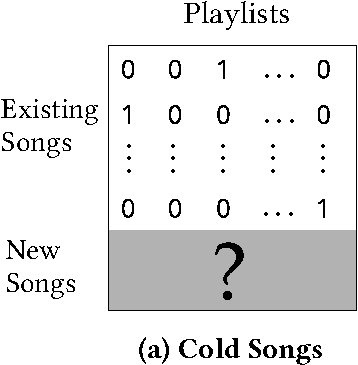
\includegraphics[width=.73\linewidth]{fig/fig_nsr.pdf}
%  \caption{}
  \label{fig:nsr}
\end{subfigure}%
\begin{subfigure}{.5\columnwidth}
  \centering
  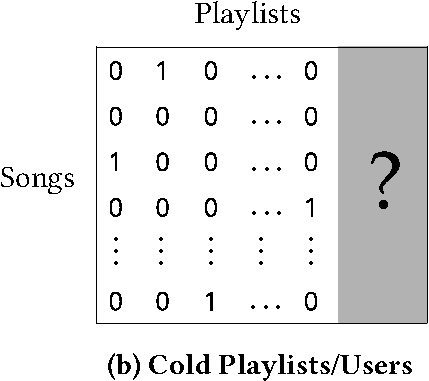
\includegraphics[width=.85\linewidth]{fig/fig_gen.pdf}
%  \caption{b}
  \label{fig:gen}
\end{subfigure}
\caption{Illustration of three cold-start settings}
\label{fig:settings}
\end{figure}


%\begin{figure}[h]
%\centering
%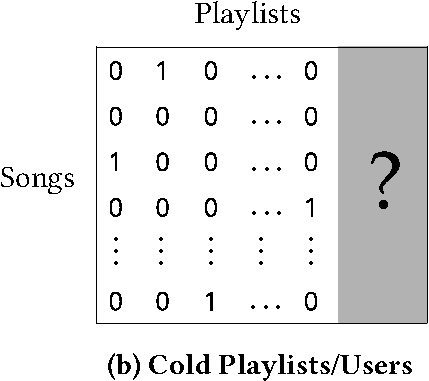
\includegraphics[width=.45\linewidth]{fig/fig_gen.pdf}
%\caption{Illustration of setting (ii) and (iii)}
%\label{fig:hr0}
%\end{figure}



%It is challenging to learn an affinity function $f$ that can deal the three cold-start settings simultaneously.
%In this next section, we propose a multitask objective which provides a function as required here.
